\documentclass[11pt,a4paper]{article}

\usepackage[margin=2.3cm]{geometry}
\usepackage[T1]{fontenc}
\usepackage{lmodern}
\usepackage{microtype}
\usepackage{amsmath,amssymb}
\usepackage{booktabs}
\usepackage{tabularx}
\usepackage{multirow}
\usepackage{enumitem}
\usepackage{caption}
\usepackage{placeins}
\usepackage{xcolor}
\usepackage{tikz}
\usetikzlibrary{arrows.meta,positioning}
\usepackage[hidelinks]{hyperref}

\setlist{itemsep=2pt,topsep=4pt}
\makeatletter   % float pages: stack from the top instead of spreading tables over the page
\setlength\@fptop{0pt}\setlength\@fpsep{14pt plus 2pt}\setlength\@fpbot{0pt plus 1fil}
\makeatother
\newcommand{\code}[1]{\texttt{#1}}
\newcolumntype{L}{>{\raggedright\arraybackslash}X}

\title{Improving the Semantic Teachers:\\[2pt]
\large Diagnosis, Ground-Truth Check and Three Teacher Variants (A, B, C)}
\author{Suhan --- Team Radiance, Department of Computer Science and Engineering,\\University of Moratuwa}
\date{8 October 2026}

\begin{document}
\maketitle

\begin{abstract}
Our semantic layer attaches CLIP and DINOv2 features to a frozen 3D Gaussian Splat so that a phrase resolves to a
3D goal. After the Phase~5 evaluation the training-free \emph{lift} found 62--63\,\% of the annotated objects.
This report investigates why the rest were missed and what improves it. A diagnostic that follows the CLIP
relevancy of each query from the 2D teacher maps into 3D shows that the lift itself loses almost nothing; about
a third of the misses come from the way the CLIP teacher averages crop scales, and about half are objects CLIP
does not recognise at all. A ground-truth check corrected two of our own annotation errors. We then tested three
teacher variants, each rebuilt end to end on two scenes and four backends: \textbf{(A)} multi-scale CLIP with the
scale chosen per query, \textbf{(B)} region-level CLIP from SAM segments, and \textbf{(C)} a larger CLIP
(ViT-L/14). Only A improved the lift (22 of 29 objects found, against 20 for the original teachers, 19 for B and
18 for C); none improved the trained FMGS field. A has been merged and is now the default lift.
\end{abstract}

\tableofcontents

%=======================================================================================
\section{Starting point}
%=======================================================================================

Each training photo of a scene is turned into \emph{teacher} feature maps: CLIP (ViT-B/16) for language and
DINOv2 for object structure. The CLIP map is built LERF/FMGS-style: square crops at seven scales (5--50\,\% of the
image's short side) are embedded, each scale is resampled onto a common grid ($\approx71\times40$ cells), and the
seven scales are \textbf{averaged with equal weight}. These maps are then attached to the Gaussians either by the
\emph{lift} (a blend-weighted average over all views, no training) or by \emph{FMGS} (a hash-grid feature field
trained against the maps). A query computes LERF relevancy per Gaussian, keeps those above a threshold relative to
the query's own peak (with a fixed floor of 0.55), clusters them and returns the best cluster.

The Phase~5 evaluation (two scenes, \emph{backroom} and \emph{flightroom}; 29 annotated objects, 6 absent objects)
left the best backend, the lift, at 8/13 and 10/16. The question was whether the misses come from using the
teachers too coarsely.

%=======================================================================================
\section{Diagnosis: where is the signal lost?}
%=======================================================================================

For every annotated object we took the three nearest training photos where it is visible and measured the same
relevancy at three stages:
\begin{enumerate}[label=(\alph*)]
  \item the cached teacher grid at the object's pixel (our scale-averaged pyramid);
  \item[(d)] CLIP on a crop \emph{centred on the object}, at each of the seven scales (best scale kept);
  \item[(c)] the lifted 3D table, at the Gaussians within 0.25\,m of the annotation.
\end{enumerate}

\begin{table}[ht]
\centering\small
\begin{tabular}{@{}lccc@{}}
\toprule
Group & (a) teacher grid & (d) best centred scale & (c) 3D table \\
\midrule
hits (18)                & 0.682 & 0.748 (+0.066) & 0.675 ($-$0.007) \\
misses (11)              & 0.485 & 0.577 (+0.093) & 0.517 \\
no-candidate misses (6)  & 0.439 & 0.522 (+0.083) & 0.504 \\
\bottomrule
\end{tabular}
\caption{Mean relevancy at each stage (0.5 = no preference; the query's floor is 0.55).}
\end{table}

\begin{itemize}
  \item \textbf{Lifting into 3D loses almost nothing} ($-0.007$ for hits): the loss happens in 2D.
  \item \textbf{Scale averaging costs 0.07--0.09 relevancy everywhere.} A 5\,\% crop around a small object is
        averaged with crops covering half the image, which dilutes it. Four misses clear 0.6 at their best
        centred scale but not on the grid (swivel chair, camera tripod, white bucket, glass door cabinet): these
        are \emph{coarseness} misses.
  \item \textbf{Recognition misses:} keyboard, floor lamp, armchair and purple foam mat stay below 0.55 even with a
        centred crop at the best scale --- finer use of the same CLIP cannot fix them.
  \item \textbf{No single scale is right:} large objects peak at the 0.5 scale (bins, mats, cart), small ones at
        0.05--0.2 (cup, clock, bucket). The scale has to be chosen per query.
\end{itemize}

%=======================================================================================
\section{Ground-truth check}
%=======================================================================================

Before changing the method we re-examined every miss by drawing the annotation and the model's top candidate
into training photos. Two misses were errors in our own annotations:
\begin{itemize}
  \item \textbf{purple foam mat:} the annotation, placed from sparse SfM points, had leaked through to points 2\,m
        behind the mat (5.2\,m depth instead of 3.1\,m). The model's ``wrong object'' was in fact the mat.
  \item \textbf{glass door cabinet:} the upper wall cabinets also have glass doors and had not been annotated as
        instances; the model's candidate was 0.2\,m from one of them.
\end{itemize}
Both were re-placed from the splat's own rendered depth, independently of the model's output. The original
frozen set and its results were kept; the corrected (\emph{amended}) set raised the lift on backroom from 8/13 to
10/13 and is used for everything below. The remaining nine genuine misses were confirmed by eye (e.g.\ the
armchair is correctly annotated but hidden behind a whiteboard in most photos).

%=======================================================================================
\section{The three variants}
%=======================================================================================

Each variant changes \emph{only how the CLIP teacher maps are made}; DINOv2, the lift, FMGS, the query and the
evaluation are identical. Each was rebuilt on both scenes for four backends: lift with CLIP (L-C), lift with
DINO at query time (L-CD), FMGS on CLIP alone (F-C) and FMGS with its paper losses (F-CD).

\begin{figure}[ht]
\centering
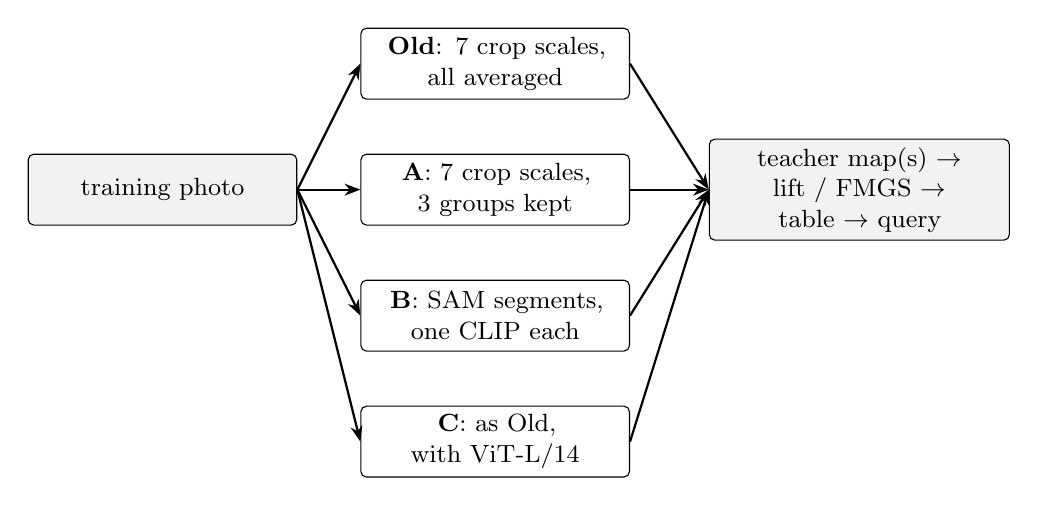
\begin{tikzpicture}[node distance=4mm and 5mm,
  box/.style={draw, rounded corners=2pt, align=center, font=\small, minimum height=9mm, inner sep=3pt, text width=3.2cm},
  arr/.style={-{Stealth[length=2mm]}, thick}]
  \node[box, fill=gray!10] (img) {training photo};
  \node[box, right=8mm of img, yshift=16mm] (old) {\textbf{Old}: 7 crop scales,\\all averaged};
  \node[box, right=8mm of img, yshift=0mm] (a) {\textbf{A}: 7 crop scales,\\3 groups kept};
  \node[box, right=8mm of img, yshift=-16mm] (b) {\textbf{B}: SAM segments,\\one CLIP each};
  \node[box, right=8mm of img, yshift=-32mm] (c) {\textbf{C}: as Old,\\with ViT-L/14};
  \node[box, right=10mm of a, fill=gray!10, text width=3.6cm] (out) {teacher map(s) $\rightarrow$\\lift / FMGS $\rightarrow$ table $\rightarrow$ query};
  \foreach \n in {old,a,b,c} { \draw[arr] (img.east) -- (\n.west); \draw[arr] (\n.east) -- (out.west); }
\end{tikzpicture}
\caption{What each variant changes: only the CLIP teacher stage.}
\end{figure}

\subsection{A --- multi-scale CLIP, scale chosen per query}
\textbf{Idea.} Keep the information that averaging throws away, and let each query pick the scale that suits its
object --- what LERF does.\\
\textbf{How.} The same seven crop scales are embedded (so the teacher cost is unchanged), but grouped into
\emph{small} ($<$\,15\,\% of the short side), \emph{medium} (15--40\,\%) and \emph{large} ($>$\,40\,\%), each group
averaged on its own. The lift attaches each group to the Gaussians separately (the overall mean follows by
linearity), and the table carries three CLIP blocks. At query time relevancy is computed per group and the group
whose top relevancies peak highest is used. For FMGS, the field gets one CLIP head per group and each training
step trains one randomly chosen group.

\subsection{B --- region-level CLIP from SAM segments}
\textbf{Idea.} Give CLIP whole objects instead of square windows that mix an object with its surroundings
--- what LangSplat does.\\
\textbf{How.} SAM (ViT-B) segments each photo with its automatic mask generator. Each segment is cut out (its
bounding box plus 10\,\% context, everything outside the mask blacked out, centred on a square) and embedded with
CLIP. Every cell of a two-times finer grid gets the coverage-weighted mean of the embeddings of the segments
covering it, so the features follow object outlines. Cells that no segment covers stay zero.

\subsection{C --- a larger CLIP}
\textbf{Idea.} Target the recognition misses directly with a stronger model.\\
\textbf{How.} The original pyramid with OpenCLIP ViT-L/14 (LAION-2B, 768-d) instead of ViT-B/16 (512-d); the query
encodes text with the same model. Everything else, including the relevancy floor and temperature, is unchanged.

%=======================================================================================
\section{Results}
%=======================================================================================

\begin{table}[ht]
\centering\small
\begin{tabular}{@{}lcccc@{}}
\toprule
 & \multicolumn{4}{c}{Top-1 hits: backroom /13 + flightroom /16 = total /29} \\
\cmidrule(l){2-5}
Teachers & Lift L-C & Lift L-CD & FMGS F-C & FMGS F-CD \\
\midrule
Old (averaged pyramid)  & 10+10 = 20 & 10+10 = 20 & 7+8 = 15 & 7+4 = 11 \\
\textbf{A multi-scale}  & \textbf{9+13 = 22} & \textbf{10+12 = 22} & 7+8 = 15 & 4+4 = 8 \\
B SAM regions           & 8+11 = 19 & 8+7 = 15 & 8+1 = 9 & 6+0 = 6 \\
C ViT-L/14              & 8+10 = 18 & 8+9 = 17 & 4+4 = 8 & 3+1 = 4 \\
\bottomrule
\end{tabular}
\caption{The four teacher settings on the amended query sets. L = lift, F = FMGS; C = CLIP only, CD = with DINOv2.}
\label{tab:main}
\end{table}

\begin{table}[ht]
\centering\small
\begin{tabular}{@{}lcccc@{}}
\toprule
Teachers (backroom / flightroom) & Teachers (min) & Lift (min) & FMGS F-CD (min) & Lift table (GB) \\
\midrule
Old  & 31 / 50   & 3.0 / 4.4   & 31 / 25 & 0.92 / 0.66 \\
A    & 32 / 53   & 17.4 / 22.6 & 31 / 25 & 2.48 / 1.77 \\
B    & 38 / 45   & 2.8 / 4.3   & 31 / 25 & 0.92 / 0.66 \\
C    & 216 / 363 & 3.7 / 5.4   & 43 / 34 & 1.18 / 0.84 \\
\bottomrule
\end{tabular}
\caption{Build cost on the RTX 2080 (8 GB). Teacher extraction is shared by every backend of a variant.}
\end{table}

\begin{table}[ht]
\centering\small
\begin{tabularx}{\linewidth}{@{}lcccL@{}}
\toprule
Lift (L-C) & Median err.\ (m) & Absent: AUROC & Peak VRAM (GB) & Changes vs Old (per query) \\
\midrule
Old  & 0.19 / 0.22 & 0.85 / 0.90 & 7.4 / 2.4 & --- \\
A    & 0.21 / 0.25 & 0.87 / 0.90 & 0.8 / 0.8 & +armchair, +upholstered chair, +water jug; $-$hose reel \\
B    & 0.15 / 0.26 & 0.80 / 0.98 & 3.6 / 2.0 & +armchair, +upholstered chair, +water jug; $-$office chair, $-$hose reel, $-$round table, $-$PVC frame \\
C    & 0.17 / 0.28 & 0.77 / 0.96 & 4.6 / 2.4 & $-$office chair, $-$purple foam mat \\
\bottomrule
\end{tabularx}
\caption{Lift details (backroom / flightroom). AUROC: how well the peak relevancy separates present from absent
objects (1 = perfectly).}
\end{table}

\FloatBarrier
\subsection{What the results mean}
\begin{itemize}
  \item \textbf{A is the only variant that improves the lift} (+2 net: 3 objects gained, 1 lost), including the
        heavily occluded armchair. This supports the diagnosis: choosing the crop scale per query recovers small
        or partly visible objects that averaging dilutes. On 29 queries the gain is encouraging but not
        statistically strong (sign test $p\approx0.3$). Its cost is a 4--5$\times$ longer lift and 2.7$\times$
        larger tables; the teacher time is unchanged and the lift's GPU peak drops, because the larger
        accumulators are kept in host memory.
  \item \textbf{No variant helps FMGS.} With A, the per-group heads split the field's capacity and F-CD falls from
        11 to 8. With B, FMGS collapses on flightroom (15 of 16 queries without a candidate): the zero vectors in
        cells no segment covers become training targets, and the field learns them. The lift simply ignores
        such cells.
  \item \textbf{B helps occluded objects but hurts thin ones.} Its object-shaped features find the armchair and the
        water jug, but segments of thin structures (PVC frame, round table) are poor CLIP inputs. It separates
        absent objects best on flightroom (AUROC 0.98).
  \item \textbf{C is not a clean negative.} The query's floor (0.55) and temperature were fixed on ViT-B/16, and
        ViT-L/14's similarities sit on a different scale, so it was judged with mis-calibrated settings --- yet it
        rejects absent objects well (0.96 on flightroom). Its teachers are 6--7$\times$ slower, and its FMGS had to
        fall back to PyTorch heads because tiny-cuda-nn ran out of memory with 768-wide outputs.
\end{itemize}

%=======================================================================================
\section{Decision and next steps}
%=======================================================================================

\textbf{Decision (8 October):} variant A was merged, and the lift now uses multi-scale teachers by default. FMGS
keeps the original scale-averaged teachers. The official lift tables of both scenes were rebuilt; the old ones
are kept for comparison. B and C remain on their own branches.

\textbf{What would make the others fair, or better:}
\begin{enumerate}
  \item \textbf{C:} recalibrate the relevancy floor on the development set for ViT-L/14, then re-evaluate --- the
        only variant aimed at the recognition misses.
  \item \textbf{B:} mask uncovered cells out of FMGS's loss, and combine segments with the pyramid where SAM
        produces no segment or only fragments of thin objects.
  \item \textbf{A + B or A + C:} the improvements target different failures (scale vs.\ object shape vs.\
        recognition) and could be combined.
  \item \textbf{More evidence:} additional scenes and queries, since a two-object difference on 29 queries is
        within noise.
\end{enumerate}

\end{document}
